\part{Umsetzung}
\begin{frame}[fragile]{Technische Realisierung}
\begin{minipage}{0.5\textwidth}
	{\setstretch{1.0}
		\begin{itemize}[itemsep=1mm]
			\item Unity, Vuforia, C\# und Python
			\item Positionierung initial über optischen Marker, danach über Spatial Mapping			
			\item Server mit Pyhton auf Basis von zwei kommunizierenden Threads
			\item Steuerung über Menu und Einstellungen via Cursor
			\item Verdeckung anhand nachmodellierter Spule
		\end{itemize}
	}
\end{minipage}
\begin{minipage}{0.45\textwidth}
	\centering
	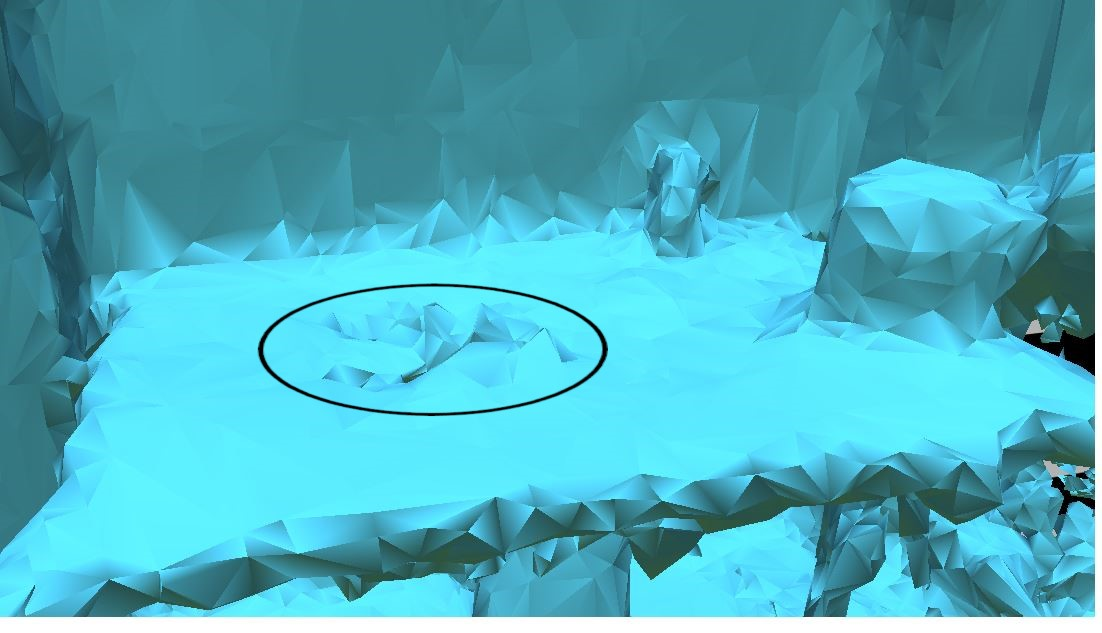
\includegraphics[width=0.8\textwidth]{images/HL/mesh.JPG}\\
	\scriptsize Spatial Mapping des Versuchsaufbaus.
	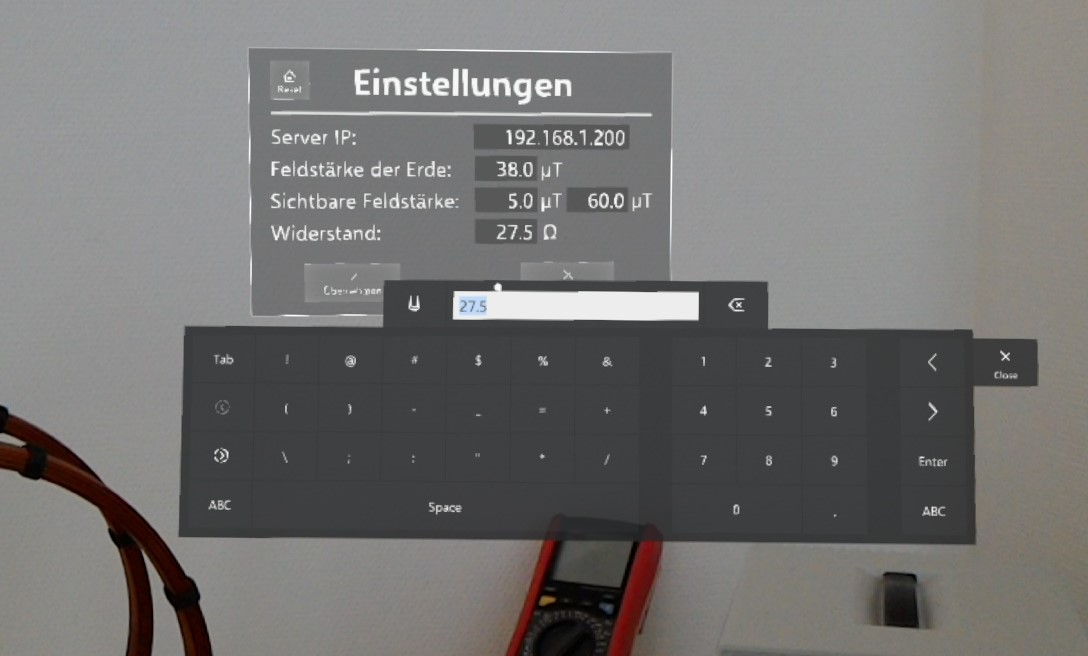
\includegraphics[width=0.8\textwidth]{images/HL/settings_c.jpg}\\
	\scriptsize Einstellungen mit aktiver Tastatur.
\end{minipage}
\end{frame}

\part{Ergebnisse}
\label{part:results}
\begin{frame}[fragile]{Dargestellte Informationen}
\begin{itemize}
	\item Visualisierung der Komponenten des Magnetfeldes in zwei Darstellungen und in Echtzeit
	\item Darstellung einer vorberechneten Lösung für eine ausgewählte Ebene des Feldes der Spule
	\item Kennzeichnung der Stromrichtung
	\item Integration einer virtuellen Kompass-Skala mit Hervorhebung wichtiger Zustände
	\item Einbettung einer virtuellen Kompassnadel auf Basis theoretischer Werte
	\item Numerische Darstellung gemessener und berechneter Echtzeitdaten
\end{itemize}
\end{frame}

\begin{frame}[fragile]{Technische Bewertung}
\begin{minipage}{0.62\textwidth}
%\centering
\bgroup
\setlength\extrarowheight{1pt}
\def\arraystretch{1.1}
\begin{table}
	\centering
	\begin{tabular}{m{4.1cm}|l}
		Kriterium & Bewertung \\
		\hline
		Framerate & Optimal\\
		\hline
		Stabilität & Fast optimal\\
		\hline
		Positionierung & Fast optimal\\
		\hline
		Komfortzone & Optimal\\
		\hline
		Tiefen Wechsel & Fast optimal\\
		\hline
		FoV-Grenzen & Optimal\\
		\hline
		Input Interaction Clarity & Erfüllt\\
		\hline
		Anpassung an Nutzerposition & Optimal\\
	\end{tabular}
\end{table}
\setlength\extrarowheight{0pt}
\def\arraystretch{1}
\egroup
\end{minipage}
\begin{minipage}{0.35\textwidth}
	%	\centering
	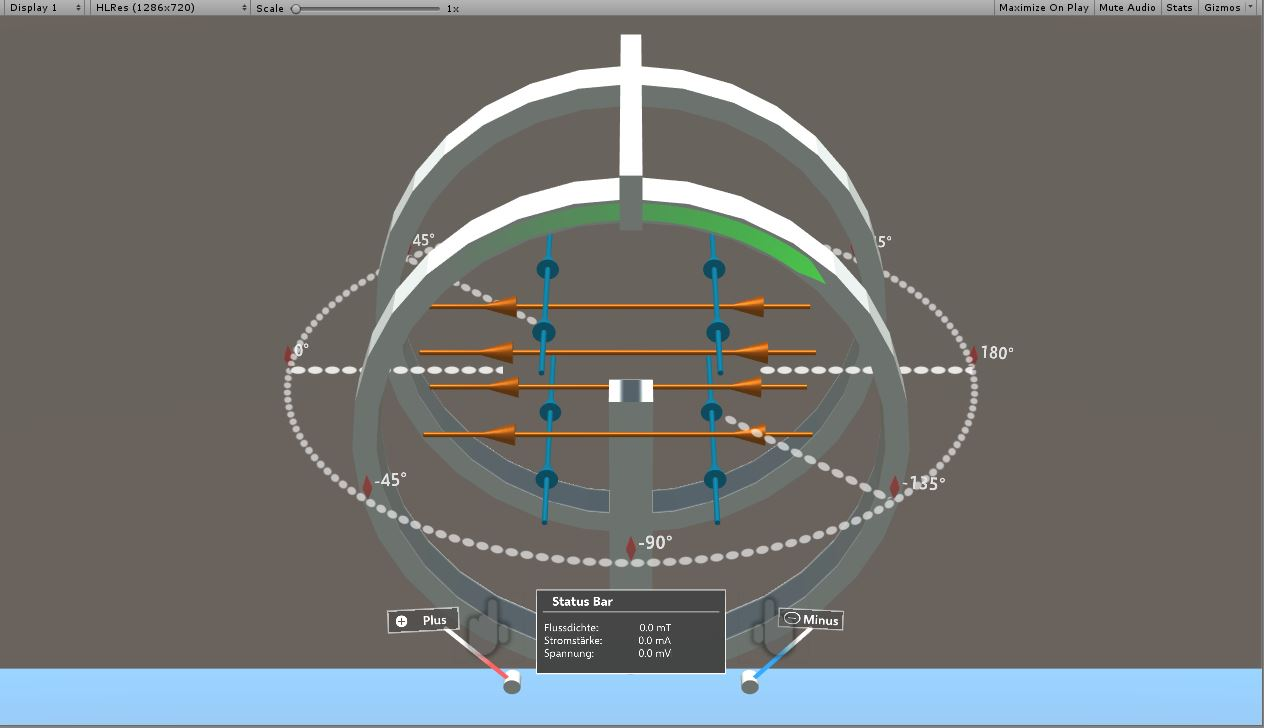
\includegraphics[width=0.98\textwidth]{images/unity/fov.JPG}\\
	
	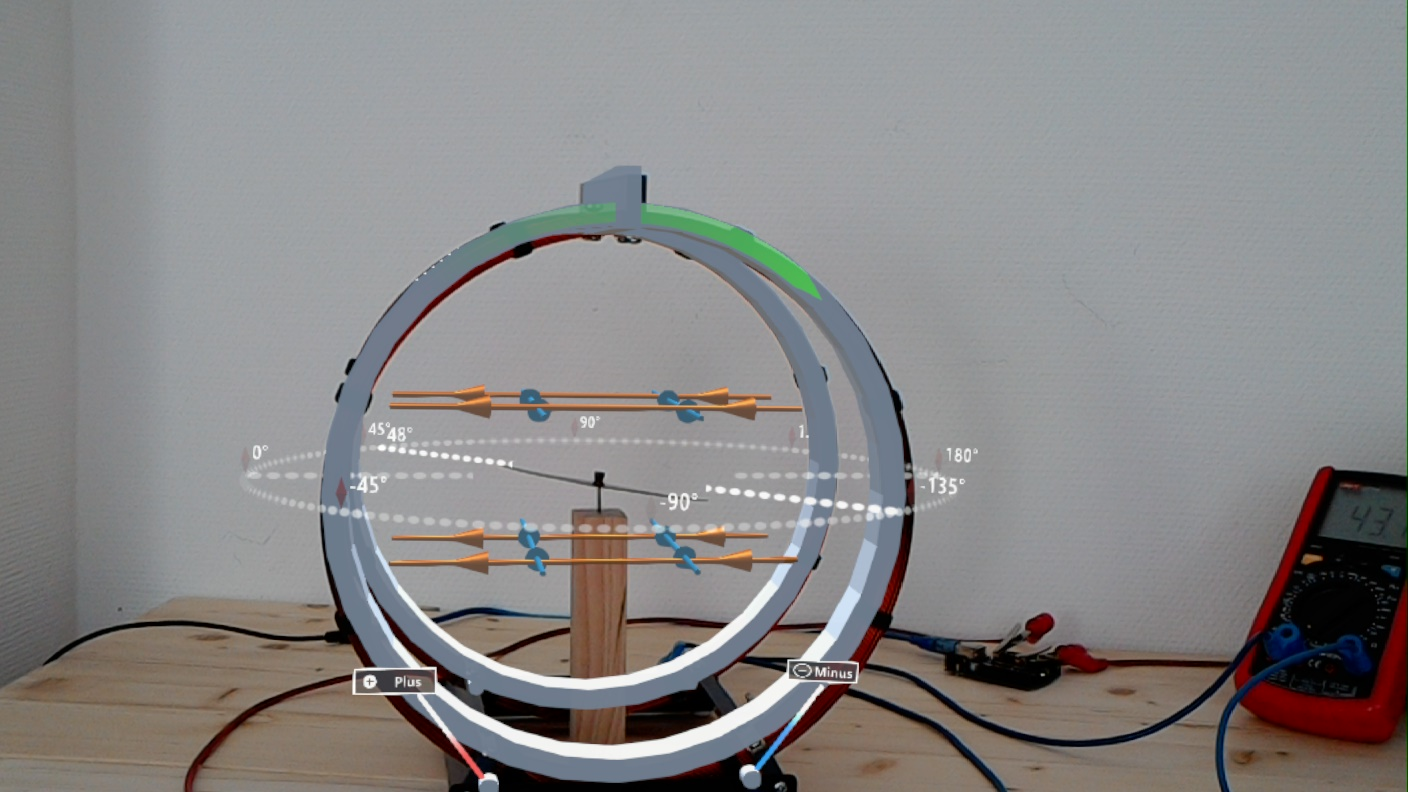
\includegraphics[width=0.98\textwidth]{images/HL/model-overlay.jpg}
\end{minipage}
% \vspace{-17px} \scriptsize \singlespacing
%Tabelle: Bewertung anhand von Qualitätskriterien. Oben: Sichtfeld bei 1,5 m Abstand. Unten: Überlagerung von Modell und Realität.
%\scriptsize Links Oben: Sichtfeld bei 1,5 m Entfernung. Links Unten: Überlagerung von Modell und Realität. Rechts: Bewertung anhand von Qualitätskriterien der Dokumentation. Stufen: ''Optimal'', ''Erfüllt'' und ''Nicht erfüllt''.
\end{frame}

\begin{frame}[fragile]{Performance}
\begin{figure}
	\vspace{-20px}
	\hspace{100px}
	\centering
	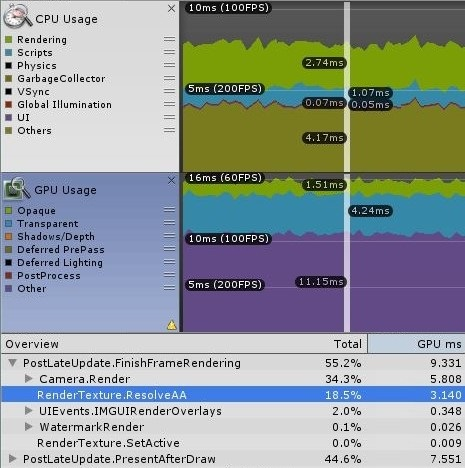
\includegraphics[width=0.6\textwidth]{images/performance/profile_MSAA_on_cut.jpg}\\
	\scriptsize Unity's Profiler zeigt Details zur Renderdauer auf CPU und GPU mit aktivem MSAA.
\end{figure}
\end{frame}

\part{Ausblick}
\label{part:future}
\begin{frame}[fragile]{Erweiterungen}
\usebeamerfont{frametitle}\textcolor{blue}{Inhaltlich:} \usebeamerfont{text}\textit{Weitere Lerninhalte integrieren}
\begin{itemize}
	\item Weitere Inhalte, z.B. Rechte-Hand-Regel
	\item Weitere Experimente, z.B. Ablenkung eines Elektronenstrahles
\end{itemize}
\pause
\vskip 1em
\usebeamerfont{frametitle}\textcolor{blue}{Technisch:} \usebeamerfont{text}\textit{Portierung für HoloLens 2}
\begin{itemize}
	\item Auflösung x4 pro Auge, Sichtfeld x2 (Fläche)
	\item Tragekomfort und Interaktion verbessert
\end{itemize}

\vspace{50px}
\end{frame}



\part{Diskussion}
\begin{frame}[fragile]{}
Vielen Dank für Ihre Aufmerksamkeit!

\vspace{1em}
\hspace{1em} Fragen?
\end{frame}
